\documentclass[DIV=calc, paper=a4, fontsize=11pt, twocolumn]{scrartcl}
\usepackage{microMathematics}
\usepackage[english]{babel} % English language/hyphenation

% Begin document
\begin{document}
\maketitle
\thispagestyle{fancy} % Enabling the custom headers/footers for the first page

\begin{bf}
% This is the first part of the file about_micromath.tex
The microMathematics Plus is the
mathematical calculator on Android
oriented around a spreadsheet that
allows live editing of mathematical
identities combined with highly
accurate computations.

It is based on a powerful touch-screen
editor that allows users to create and
manipulate naturally readable
worksheets containing all basic
mathematical notations.

The microMathematics Plus supports
high school-level of mathematical
calculations. This version has
following mathematical limitations: it
does not support special functions,
vectors, matrices and many other
things from high-level mathematics.
\end{bf}

\section{How To Use}
% This is auto-generated file: do not edit!
% Exported from microMathematics Plus, version 2.16.2


This app is a powerful calculation
software in a worksheet format. The
worksheet can be freely edited, stored
on SD card, opened from SD card and
exported into an image or LaTeX
format.

Worksheet is a mathematical document
that contains text, formulas and
plots. It supports live editing of
typeset mathematical notations and its
automatic computation.

Following objects can be inserted into
worksheet: equations, result views,
plots, text fragments and images. This
document gives an overview on how to
edit these objects.

\subsection{Editing}

Almost all available objects contain
several editable fields. To edit the
field use the symbols and functions on
the tool bar.

All symbols can also be entered from
the keyboard. To find out which
keyboard symbol corresponds to the
mathematical symbol you want to enter,
read the hint by long click on the
button of interest.

Using long click on a term you can
select this term. The selected term
can be deleted, copied to clipboard,
pasted from clipboard or an other
operator or function can be inserted
after that term using buttons from the
tool bar or keyboard.

The ''Undo'' command is available in the
action bar. It erases the last change
done to the document and reverts it to
an older state:
\begin{center}\begin{tabular}{c} 
\includegraphics[resolution=320]{graphics/how_to_use_fig1.png} \end{tabular}\end{center}

\subsection{Equation}

An equation defines a numerical
constant, an interval or a function.
To create an equation, use the ''New
element'' button in the action bar
\begin{center}\begin{tabular}{c} 
\includegraphics[resolution=320]{graphics/how_to_use_fig2.png} \end{tabular}\end{center}

or the ''Add equation'' button from the
tool bar:
\begin{center}\begin{tabular}{c} 
\includegraphics[resolution=320]{graphics/how_to_use_fig3.png} \end{tabular}\end{center}

An equation with two empty fields
appears. These fields shall be filled:
\begin{center}\begin{tabular}{c}
  ${\Box} := {\Box}$
\end{tabular}\end{center}

The equation name is given in the left
field. The name shall contain letters
or digits only and will be used in
other objects in order to reference
this equation.

From the action bar, you can open
''Document settings'' dialog window: 
\begin{center}\begin{tabular}{c} 
\includegraphics[resolution=320]{graphics/how_to_use_fig4.png} \end{tabular}\end{center}

Depending on the parameter ''Allow to
re-define equations'' in this dialog,
there are two usage modes:

a) if re-definition is not allowed,
the equation name shall be unique
within whole worksheet and the
equation can be used both before and
after its definition,

b) if re-definition is allowed, you
can define more than one equation with
the same name. If such an equation is
referenced, the last version defined
before the caller equation will be
used.

\subsubsection{Constant}

If the equation name does not contain
any argument in brackets, it defines a
constant or an interval:
\begin{center}\begin{tabular}{ccc}
  $N := 200$ &
  $Sq2 := \sqrt{100} $ &
  $Pi2 := \frac{{\pi}}{2}$ \cr
\end{tabular}\end{center}

In the last example, a built-in
constant pi was used. Currently, the
following built-in constants are
available:
\begin{center}\begin{tabular}{ccc}
  ${\pi} = 3.14159$ &
  $pi = 3.14159$ &
  $e = 2.71828$ \cr
\end{tabular}\end{center}

A previously defined constant can also
be used:
\begin{center}\begin{tabular}{c}
  $NPi2 := N \cdot Pi2$
\end{tabular}\end{center}

You can also use the symbol ''i'' as
imaginary unit in order to define a
complex number:
\begin{center}\begin{tabular}{c}
  $z := 5+3i$
\end{tabular}\end{center}

\subsubsection{Units}

If you need a unit for the constant,
you can put it from the keyboard into
the same input field. The unit shall
be separated from the number using
space. You can use units both for real
and complex constants:
\begin{center}\begin{tabular}{ccc}
  $r := 10 m$ &
  $a := {10 m}^{2}$ &
  $v := 10 km / hr$ \cr
\end{tabular}\end{center}
\begin{center}\begin{tabular}{cc}
  ${\alpha} := 45 {\degree} + 30 ' + 15 ''$ &
  ${\varphi} := 100 \cdot \frac{kg \cdot m}{{s}^{2}}$ \cr
\end{tabular}\end{center}

The document ''units\_overview.mmt''
contains the list of all supported
units. This document is delivered with
the app and stored in ''Resources
of microMathematics Plus''.

\subsubsection{Interval}

An interval type equation defines a
variable that is changed from a given
minimum value up to a given maximum
value with defined increment. This
variable can be used as a function
plot argument or as a parameter to
build a function value table.

To define an interval, put a valid
name on the left side of an empty
equation. On the right side of this
equation, put either a symbol '':'', or
click the button ''Equidistant
interval'' from the tool bar:
\begin{center}\begin{tabular}{c} 
\includegraphics[resolution=320]{graphics/how_to_use_fig5.png} \end{tabular}\end{center}

Here, the first element is the interval
start point, the next element is the
second point, and the last element is
the interval end point:
\begin{center}\begin{tabular}{c}
  $x := \left[ 0,\, 0.1 \,..\, 10 \right]$
\end{tabular}\end{center}

The interval elements shall be accessed
by index:
\begin{center}\begin{tabular}{ccc}
  $x_{0}  = 0.0$ &
  $x_{1}  = 0.1$ &
  $x_{100}  = 10.0$ \cr
\end{tabular}\end{center}

The increment is the difference between
two neighbours values:
\begin{center}\begin{tabular}{c}
  $x_{2}  - x_{1}  = 0.1$
\end{tabular}\end{center}

For example, we can define an
equidistant interval that contains N
points distributed with increment ''dy''
where the interval start is zero as
follows:
\begin{center}\begin{tabular}{cc}
  $dy := 0.05$ &
  $y := \left[ 0,\, dy \,..\, dy \cdot N \right]$ \cr
\end{tabular}\end{center}

\subsubsection{Function}

A function is a relation between one or
more arguments and a set of
permissible outputs with the property,
that each argument value (real or
complex) or arguments combination is
related to exactly one output.

The function name and the function
argument in brackets are given on the
left side of an equation. It is not
necessary to define the argument in
the worksheet previously, you can
define it as you want, but using
letters or digits only:
\begin{center}\begin{tabular}{c}
  $f(t) := sin \left( t\right)  \cdot cos \left( t\right)  / 2$
\end{tabular}\end{center}
\begin{center}\begin{tabular}{c}
  $w(z) := {e}^{2i \cdot {\pi} \cdot z}$
\end{tabular}\end{center}
\begin{center}\begin{tabular}{c}
  $H(x,y) := \sqrt{{x}^{2} + {y}^{2}} $
\end{tabular}\end{center}
\begin{center}\begin{tabular}{c}
  $g(x,y) := \frac{sin \left( H \left( x,\, y\right) \right) }{H \left( x,\, y / 2\right)  + 1}$
\end{tabular}\end{center}

The right side of the function contains
a mathematical formula how to
calculate the function. If this
formula does not contain the declared
function argument, such a function
will be interpreted as a constant.

You can also use on the right side
other built-in or previously defined
functions. To insert a function enter
its name, click the left bracket
symbol ''('' and than enter its
argument. This argument can also be a
formula, which contains any other
operations and functions.

The document ''functions\_overview.mmt'',
stored within the ''Resources of
microMathematic Plus'', provides the
list of all available functions.

\subsubsection{Array}

Arrays are special functions with
following properties:

a) only a previously defined interval
can be used as array argument:
\begin{center}\begin{tabular}{cc}
  $k := \left[ 0,\, 1 \,..\, 100 \right]$ &
  $m := \left[ 0,\, 1 \,..\, 200 \right]$ \cr
\end{tabular}\end{center}

a) array arguments are given in [ ]
instead of ( ):
\begin{center}\begin{tabular}{c}
  $M[k,m] := {sin \left( k / 10\right) }^{2} - 3 \cdot  \left| cos \left( m / 10\right)  \right| $
\end{tabular}\end{center}

c) array elements are calculated and
stored in memory that reduces the
access time to these values

d) array elements can be only accessed
by using a lower index. To create
lower index, put ''['' after the array
name:
\begin{center}\begin{tabular}{cc}
  $M_{5,\, 10}  = -1.39106$ &
  $M_{10,\, 5}  = -1.92467$ \cr
\end{tabular}\end{center}
\begin{center}\begin{tabular}{c}
  $N[k,m] := floor \left( -10 \cdot M_{k,\, m} \right) $
\end{tabular}\end{center}

e) if any array index is complex or
negative or greater than the upper
bound of the corresponding interval,
the invalid number will be returned:
\begin{center}\begin{tabular}{cc}
  $M_{10i,\, 100}  = NaN$ &
  $M_{90,\, 210}  = NaN$ \cr
\end{tabular}\end{center}

\subsection{Result View}

This element is aimed to represent a
calculation result as a number or a
table. To add this element, use the
''New element'' button on the action bar
or the ''Add result view'' button from
the tool bar:
\begin{center}\begin{tabular}{c} 
\includegraphics[resolution=320]{graphics/how_to_use_fig6.png} \end{tabular}\end{center}

An equation with two fields appears,
where the left field shall be filled:
\begin{center}\begin{tabular}{c}
  ${\Box} = {\Box}$
\end{tabular}\end{center}

The left term contains a formula to be
calculated and the right term is the
calculation result. The result will be
shown when you press the floating
button ''Calculate''.

Within the left term you can use any
constants and functions defined
previously as well as any built-in
functions:
\begin{center}\begin{tabular}{c}
  ${e}^{{\pi}} \cdot f \left( NPi2\right)  = 2.27286E-14$
\end{tabular}\end{center}

If the left part does not contain any
''interval-like'' variables, the
calculation result is just a real or
complex number:
\begin{center}\begin{tabular}{c}
  $y_{N - 1}  - y_{0}  = 9.95$
\end{tabular}\end{center}
\begin{center}\begin{tabular}{ccc}
  $\Re\left( z \right)  = 5.0$ &
  $\Im\left( z \right)  = 3.0$ &
  $ \left| z \right|  = 5.83095$ \cr
\end{tabular}\end{center}
\begin{center}\begin{tabular}{c}
  $\sqrt{sin \left( \frac{3}{2} \cdot {\pi}\right) }  = 0.0+1.0i$
\end{tabular}\end{center}

If the left part contains any variable
that has a dimensional unit, than the
result can have dimension as well:
\begin{center}\begin{tabular}{c}
  $2 \cdot {\alpha} / 10 s = 0.15884 rad/s$
\end{tabular}\end{center}

If the left part contains an interval
variable, the calculation result is a
vector of values corresponding to this
interval. Due to free space limit on
the display, only the first six and
the last elements of the vector will
be displayed:
\begin{center}\begin{tabular}{ccc}
  $x = \begin{bmatrix}0.0\\0.1\\0.2\\0.3\\0.4\\0.5\\\dots\\10.0\\\end{bmatrix}$ &
  $y = \begin{bmatrix}0.0\\0.05\\0.1\\0.15\\0.2\\0.25\\\dots\\10.0\\\end{bmatrix}$ &
  $2 \cdot y = \begin{bmatrix}0.0\\0.1\\0.2\\0.3\\0.4\\0.5\\\dots\\20.0\\\end{bmatrix}$ \cr
\end{tabular}\end{center}
\begin{center}\begin{tabular}{c}
  $N_{k,\, m}  = \begin{bmatrix}30.0&29.0&29.0&28.0&\dots&12.0\\29.0&29.0&29.0&28.0&\dots&12.0\\29.0&29.0&29.0&28.0&\dots&11.0\\29.0&28.0&28.0&27.0&\dots&11.0\\\dots&\dots&\dots&\dots&\dots&\dots\\27.0&26.0&26.0&25.0&\dots&9.0\\\end{bmatrix}$
\end{tabular}\end{center}

Number of displayed elements and the
mode in which the result is displayed
can be changed. Using the long click
on the formula area and the context
menu, select the whole formula. If the
formula is selected, the floating
button ''Object properties'' appears. If
you click this button, the result
properties dialog will be displayed:
\begin{center}\begin{tabular}{c} 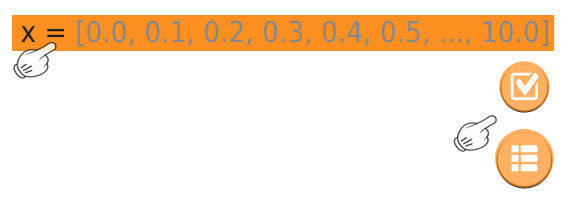
\includegraphics[resolution=320]{graphics/how_to_use_fig7.png} \end{tabular}\end{center}

The second floating button, ''Details'',
will also appear. If you click on this
button, the ''Details'' dialog will be
displayed, where you can observe all
elements of the array.

Note that the use of three or more
''interval-like'' variables on the left
part of a result view is not allowed
in this app version.

\subsection{Function Plot}

The function plot element displays a
graph of a function, which depends on
a single argument. To create a plot,
use the ''New element'' button in the
action bar or the ''Add function plot''
button from the tool bar:
\begin{center}\begin{tabular}{c} 
\includegraphics[resolution=320]{graphics/how_to_use_fig8.png} \end{tabular}\end{center}

Plot panel with six empty fields
appears. The function to be plot shall
be put in the middle-left field and
the function argument in the
middle-bottom field:
\begin{center}\begin{tabular}{c} 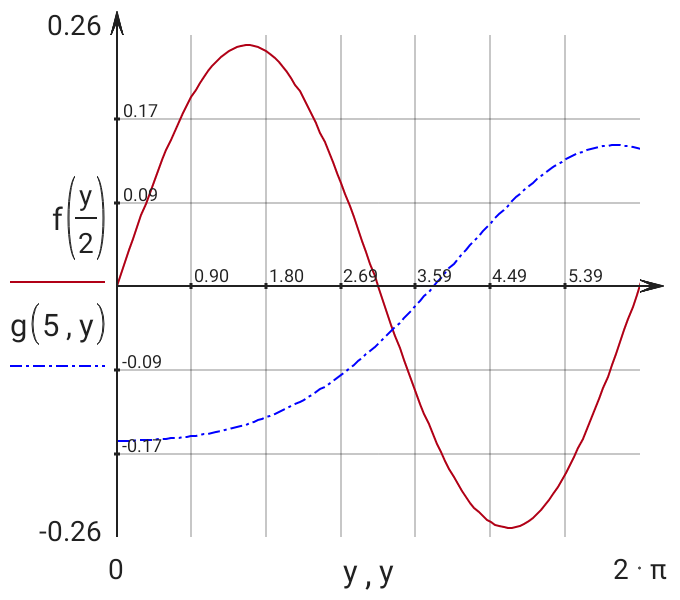
\includegraphics[resolution=320]{graphics/how_to_use_fig9.png} \end{tabular}\end{center}

For more details see ''Function Plot''
and ''Polar Function Plot'' examples
from the app navigation drawer.

\subsection{Three-dimensional Plot}

The 3D plot element displays a graph of
a single function that depends on two
arguments. To create such a plot, use
the ''New element'' button in the action
bar or the ''Add 3D plot'' button from
the tool bar:
\begin{center}\begin{tabular}{c} 
\includegraphics[resolution=320]{graphics/how_to_use_fig10.png} \end{tabular}\end{center}
\begin{center}\begin{tabular}{cc}
  $x := \left[ -10,\, -9.5 \,..\, 10 \right]$ &
  $y := \left[ -10,\, -9.5 \,..\, 10 \right]$ \cr
\end{tabular}\end{center}
\begin{center}\begin{tabular}{c} 
\includegraphics[resolution=320]{graphics/how_to_use_fig11.png} \end{tabular}\end{center}

In the center-bottom field, put the
function name or an equation that
contains exactly two previously
defined intervals. The use of an array
is also possible:
\begin{center}\begin{tabular}{c} 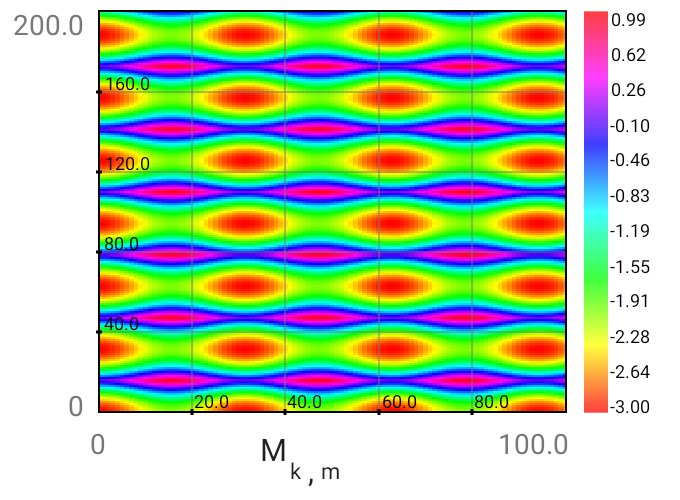
\includegraphics[resolution=320]{graphics/how_to_use_fig12.png} \end{tabular}\end{center}

For more details see ''3D Plot'' example
from the app navigation drawer.

\subsection{Text Fragment}

The text fragment element displays
simple text like this one. To add a
text fragment, use the ''New element''
button in the action bar or ''Add text
fragment'' button from the tool bar:
\begin{center}\begin{tabular}{c} 
\includegraphics[resolution=320]{graphics/how_to_use_fig13.png} \end{tabular}\end{center}

If the whole text within a fragment is 
selected using the context menu
''Select all'', a floating button
''Object properties'' appears in the
bottom-right of the screen.

If you click on this button, the ''Text
properties'' dialog will be displayed,
where you can select the text style
and activate the numbering. For
example, the titles in this document
have the style ''Subsection'' with
activated numbering.

\subsection{Image}

You can also insert an image from the
image file. To do it, use the ''New
element'' button from the action bar or
the ''Add image from file'' button from
the tool bar:
\begin{center}\begin{tabular}{c} 
\includegraphics[resolution=320]{graphics/how_to_use_fig14.png} \end{tabular}\end{center}

The ''Image settings'' dialog will
appear. There you can select a file
with the image to be inserted and set
the necessary image size.

The following image formats are
supported: png, bmp, gif, jpeg, svg.

If you activate the ''Embedded image''
flag in the ''Image settings'' dialog,
then the image will be embedded
directly in your document. Embedded
image results in stand-alone, but
larger document.

If the ''Embedded image'' flag is not
set, the image file will be just
referenced rather than embedded, i.e.
your document references the image
file outside the document. In case you
move your document please do not
forget to move the image file as well.

You can change the properties of an
already existing image. Long click on
the image area until the floating
button ''Object properties'' appears. If
you press this button, a dialog with
image properties will be displayed.

\section{Example: Function Plot}
% This is auto-generated file: do not edit!
% Exported from microMathematics Plus, version 2.15.4


This example demonstrates how to
prepare and adjust a graphical
representation of a function. For
example, we want to plot three
different functions:
\begin{center}\begin{tabular}{c}
  $f(x) := 25 + 10 \cdot sin \left( \sqrt{ \left| x \right| } \right) $
\end{tabular}\end{center}
\begin{center}\begin{tabular}{c}
  $g(x) := \frac{2}{{e}^{ \left| x \right|  / 15}} \cdot f \left( x \cdot 50\right) $
\end{tabular}\end{center}
\begin{center}\begin{tabular}{c}
  $h(x) := min \left( f \left( x\right) ,\, g \left( x\right) \right) $
\end{tabular}\end{center}

The function argument that represents
the x-values will be taken for N
points within the interval [x1, x2]:
\begin{center}\begin{tabular}{ccc}
  $N := 300$ &
  $x1 := -30$ &
  $x2 := 30$ \cr
\end{tabular}\end{center}
\begin{center}\begin{tabular}{c}
  $x := \left[ x1,\, x1 + \left( x2 - x1 \right) / N \,..\, x2 \right]$
\end{tabular}\end{center}

After the functions and their arguments
are defined, you can add the plot box
using the ''New element'' button in the
action bar or ''Add function plot''
button from the tool bar:
\begin{center}\begin{tabular}{c} 
\includegraphics[resolution=320]{graphics/function_plot_fig1.png} \end{tabular}\end{center}
\begin{center}\begin{tabular}{c} 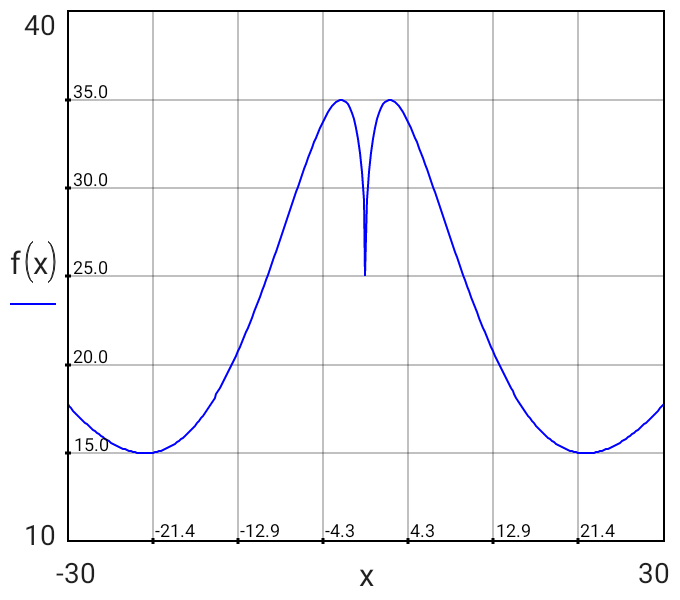
\includegraphics[resolution=320]{graphics/function_plot_fig2.png} \end{tabular}\end{center}

The function to be plotted will be put
in the middle-left field. It can also
be a built-in or previously declared
function as well as a mathematical
expression that contains any other
operators and functions.

The function input, which represents
the x-values will be put in the
middle-bottom field. It can be a
variable of interval type or a
mathematical expression that contains
an interval variable.

All other four fields describe the
plot boundaries. If these elements
remain empty, the program will
calculate corresponding values
automatically. However, you can edit
these fields at any time and put there
the values you want.

You can plot several functions on the
same plot view. To add an other
function, select the function (by long
click in the middle-left field) after
which an other function shall be added
and press ''Add new argument'' button
from the tool bar:
\begin{center}\begin{tabular}{c} 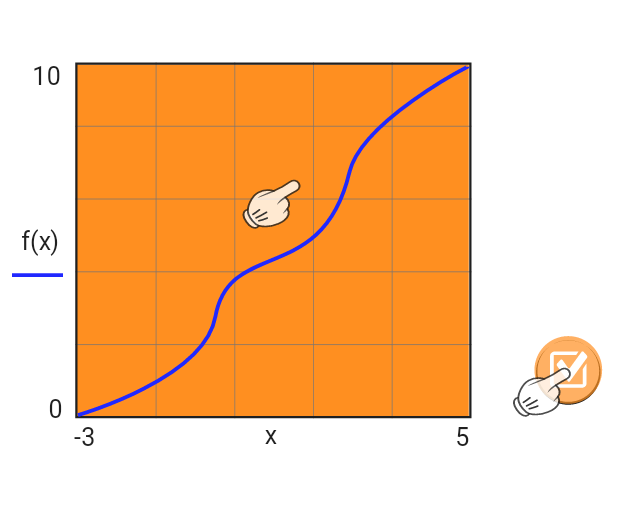
\includegraphics[resolution=320]{graphics/function_plot_fig3.png} \end{tabular}\end{center}
\begin{center}\begin{tabular}{c} 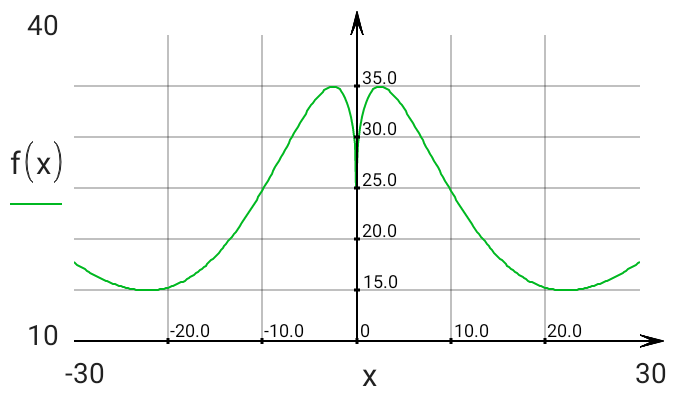
\includegraphics[resolution=320]{graphics/function_plot_fig4.png} \end{tabular}\end{center}

By long click on the middle of plot
area, the context menu and the
floating button ''Object properties''
will appear.
\begin{center}\begin{tabular}{c} 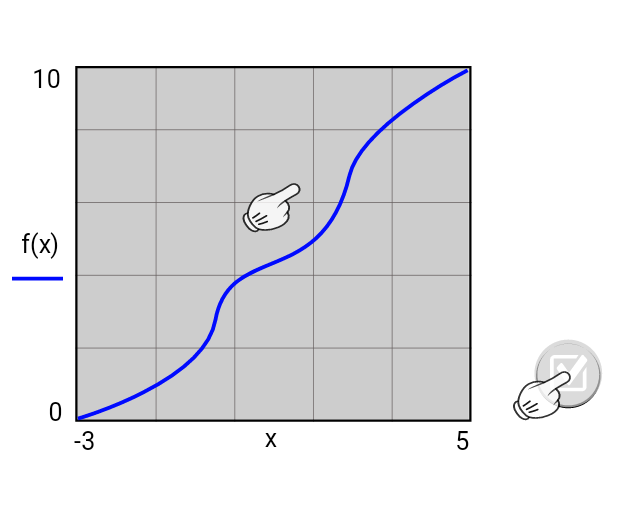
\includegraphics[resolution=320]{graphics/function_plot_fig5.png} \end{tabular}\end{center}

If you press this floating button, the
''Plot Settings'' dialog will be
displayed. Here, you can change size
and style of the plot area. For
example, the crossed graph looks like
this:
\begin{center}\begin{tabular}{c} 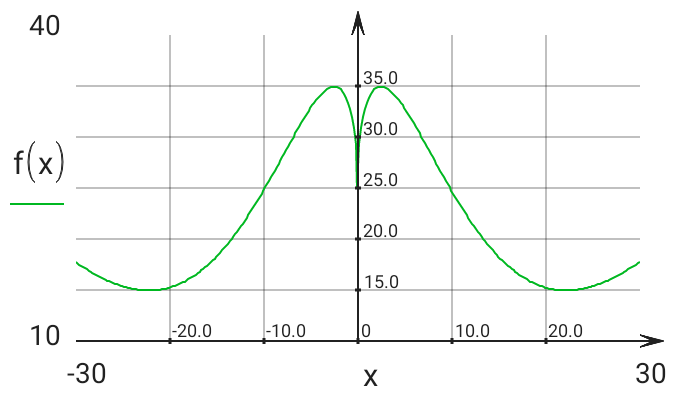
\includegraphics[resolution=320]{graphics/function_plot_fig6.png} \end{tabular}\end{center}

You can also change the plot line
color, width and style in the ''Line
Settings'' dialog. It appears by long
click on the line marker below the
function name on the left of plot
area:
\begin{center}\begin{tabular}{c} 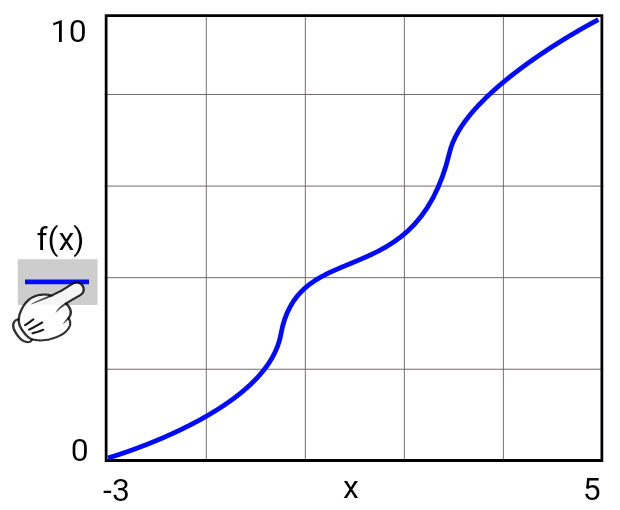
\includegraphics[resolution=320]{graphics/function_plot_fig7.png} \end{tabular}\end{center}

For example, we can use dotted lines:
\begin{center}\begin{tabular}{c} 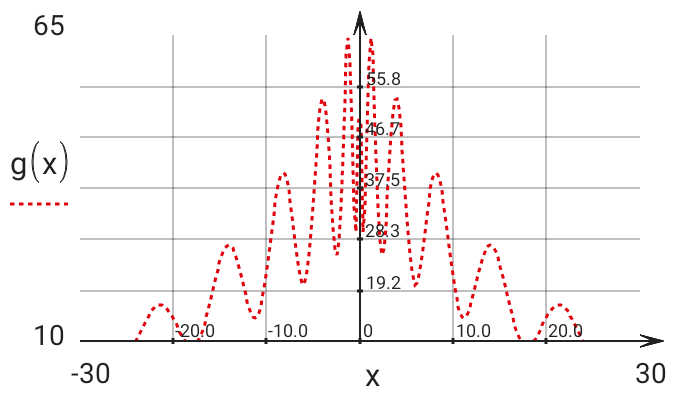
\includegraphics[resolution=320]{graphics/function_plot_fig8.png} \end{tabular}\end{center}

The number of axis labels and grid line
color can be changed in the ''Grid
Settings'' dialog. It appears by long
click on the free space between the x
minimum value (-30) and the argument
(x) symbol or between the x symbol and
the x maximum value (30) below the
plot area:
\begin{center}\begin{tabular}{c} 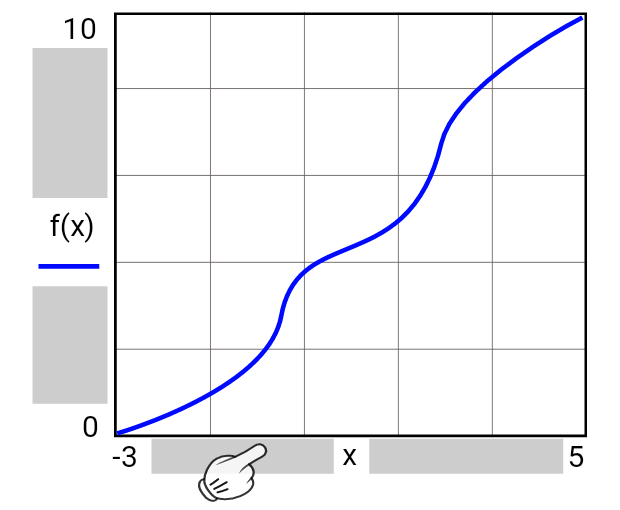
\includegraphics[resolution=320]{graphics/function_plot_fig9.png} \end{tabular}\end{center}
\begin{center}\begin{tabular}{c} 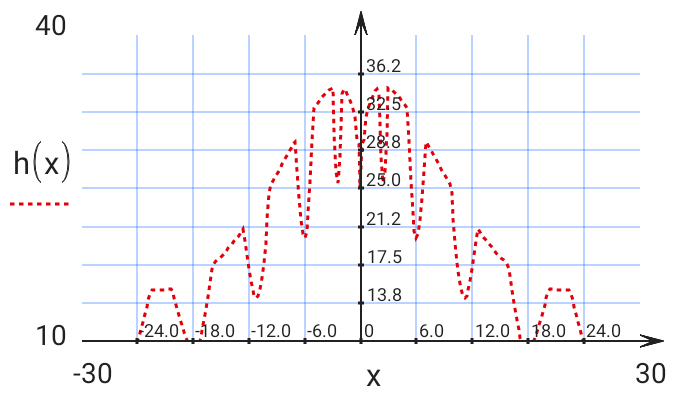
\includegraphics[resolution=320]{graphics/function_plot_fig10.png} \end{tabular}\end{center}

To hide grid completely just set the
number of grid lines to zero for both
vertical and horizontal axes.

\section{Example: Polar Function Plot}
% This is auto-generated file: do not edit!
% Exported from microMathematics Plus, version 2.17.2


Now we plot several functions given in
the polar coordinate system. Each
point in this system is determined by
a distance r from the origin and the
angle f from the x-axis.
\begin{center}\begin{tabular}{c} 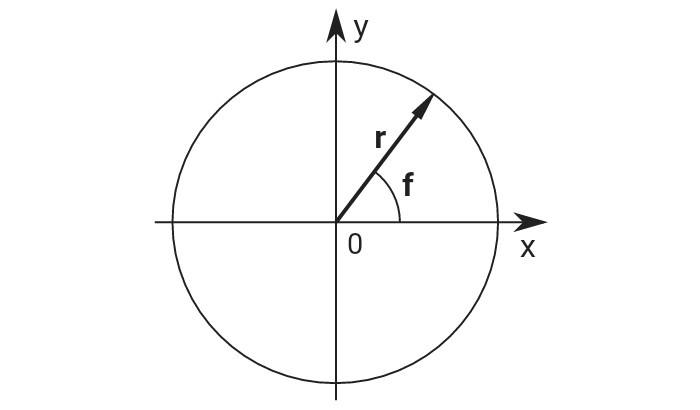
\includegraphics[resolution=320]{graphics/polar_plot_fig1.png} \end{tabular}\end{center}

The angle f is our independent variable
that is changed as follows:
\begin{center}\begin{tabular}{c}
  $f := \left[ 0.01,\, 0.05 \,..\, 300 \right]$
\end{tabular}\end{center}

The distance r(f) is our dependent
variable. Having a pair of f and r, we
can transform it to the Cartesian
coordinates x and y using sine and
cosine functions:
\begin{center}\begin{tabular}{cc}
  $x(r) := r \cdot cos \left( f\right) $ &
  $y(r) := r \cdot sin \left( f\right) $ \cr
\end{tabular}\end{center}

\subsection{A snail}

We will define our polar function in
three steps. The first expression
defines a ''wheel'':
\begin{center}\begin{tabular}{ccc}
  $A := 1.1$ &
  $B := 1.271$ &
  $q := 2$ \cr
\end{tabular}\end{center}
\begin{center}\begin{tabular}{c}
  $r1(f) := A + 2 \cdot {sin \left( B \cdot f\right) }^{q}$
\end{tabular}\end{center}

To plot this function, we add the plot
box using the ''New element'' button
in the action bar or ''Add function
plot'' button from the tool bar:
\begin{center}\begin{tabular}{c} 
\includegraphics[resolution=320]{graphics/polar_plot_fig2.png} \end{tabular}\end{center}

Instead of f and r, we use here
previously defined rules for x and y
transformation, where r1(f) is used as
a symbolic argument for these rules:
\begin{center}\begin{tabular}{c} 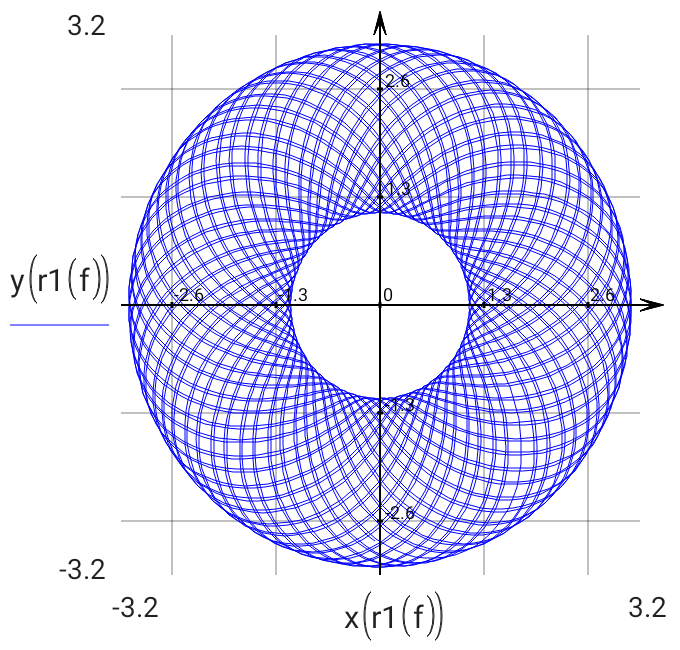
\includegraphics[resolution=320]{graphics/polar_plot_fig3.png} \end{tabular}\end{center}

Next, we can modify this wheel as
follows:
\begin{center}\begin{tabular}{c}
  $r2(f) := A + 2 \cdot {sin \left( B \cdot f + 1 \cdot r1 \left( f\right) \right) }^{q}$
\end{tabular}\end{center}
\begin{center}\begin{tabular}{c} 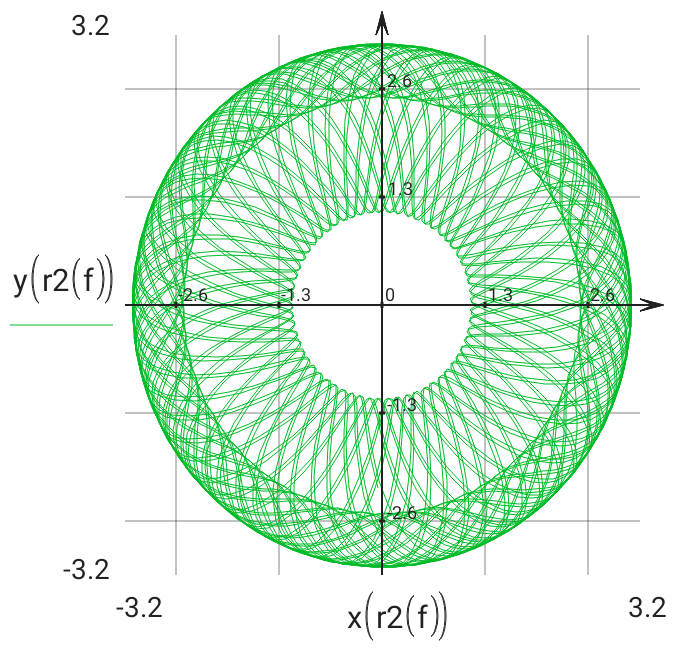
\includegraphics[resolution=320]{graphics/polar_plot_fig4.png} \end{tabular}\end{center}

Finally, we scale the last function
r2(f) using a float to integer
conversion that looks like a step
function. As a result, we obtain a
nice snail:
\begin{center}\begin{tabular}{c}
  $r(f) := r2 \left( f\right)  \cdot floor \left( f\right)  / 10$
\end{tabular}\end{center}
\begin{center}\begin{tabular}{c} 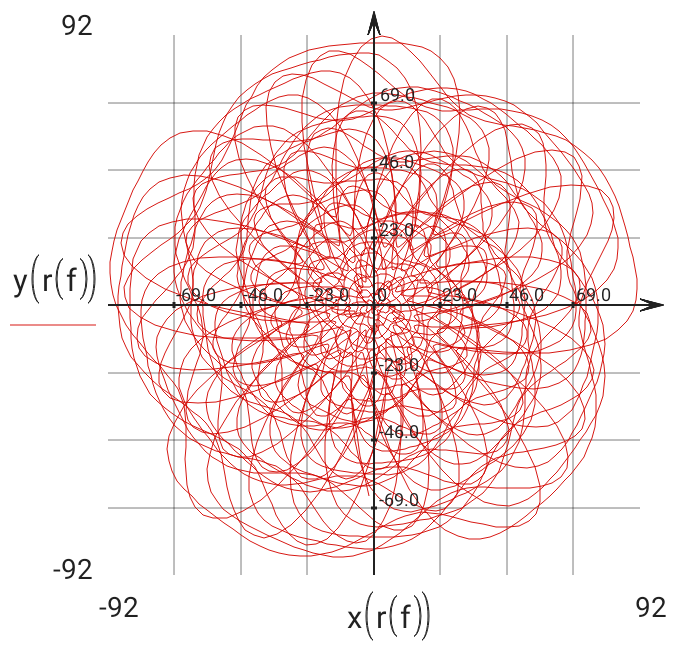
\includegraphics[resolution=320]{graphics/polar_plot_fig5.png} \end{tabular}\end{center}

\subsection{Japanese Maple}

Japanese Maple is well known for its
attractive leaf shapes and colors.
Such a leaf can be described
mathematically and plotted as a curve
in the polar coordinate system:
\begin{center}\begin{tabular}{c}
  $f := \left[ 0.01,\, 0.02 \,..\, 100 \right]$
\end{tabular}\end{center}
\begin{center}\begin{tabular}{cc}
  $x(r) := r \cdot cos \left( f\right) $ &
  $y(r) := r \cdot sin \left( f\right) $ \cr
\end{tabular}\end{center}
\begin{center}\begin{tabular}{c}
  $s1(f) := \left( 1 + sin \left( f\right)  \right) \cdot \left( 1 - 0.9 \cdot  \left| sin \left( 4 \cdot f\right)  \right|  \right)$
\end{tabular}\end{center}
\begin{center}\begin{tabular}{c}
  $s2(f) := 0.9 + 0.05 \cdot cos \left( 200 \cdot f\right) $
\end{tabular}\end{center}
\begin{center}\begin{tabular}{c}
  $r(f) := floor \left( f\right)  \cdot s1 \left( f\right)  \cdot s2 \left( f\right)  + random \left( 2\right)  - 1$
\end{tabular}\end{center}
\begin{center}\begin{tabular}{c} 
\includegraphics[resolution=320]{graphics/polar_plot_fig6.png} \end{tabular}\end{center}

http://en.wikipedia.org/wiki/Acer\_palmatum

\section{Example: 3D Plot}
% This is auto-generated file: do not edit!
% Exported from microMathematics Plus, version 2.16


This example demonstrates 3D plots for
three different functions of two
variables.

First, we define intervals for both x
and y arguments. The interval for the
x-axis depends on the number of points
along the x-axis and the minimum and
maximum values, x1 and x2:
\begin{center}\begin{tabular}{ccc}
  $N := 300$ &
  $x1 := -2$ &
  $x2 := 2$ \cr
\end{tabular}\end{center}
\begin{center}\begin{tabular}{c}
  $x := \left[ x1,\, x1 +  \left| x2 - x1 \right|  / N \,..\, x2 \right]$
\end{tabular}\end{center}

The interval for the y-axis is defined
analogously:
\begin{center}\begin{tabular}{ccc}
  $M := 300$ &
  $y1 := -3$ &
  $y2 := 3$ \cr
\end{tabular}\end{center}
\begin{center}\begin{tabular}{c}
  $y := \left[ y1,\, y1 +  \left| y2 - y1 \right|  / M \,..\, y2 \right]$
\end{tabular}\end{center}

For example, let us plot a
trigonometric function that is a
product of sine and cosine:
\begin{center}\begin{tabular}{c}
  $F(x,y) := sin \left( 3 \cdot {x}^{2}\right)  \cdot cos \left( {y}^{2}\right) $
\end{tabular}\end{center}

To create a 3D plot view, click on the
''New element'' button from the action
bar or ''Add 3D plot'' button from the
tool bar:
\begin{center}\begin{tabular}{c} 
\includegraphics[resolution=320]{graphics/three_d_plot_fig1.png} \end{tabular}\end{center}

Put the function name F(x,y) into the
center-bottom field:
\begin{center}\begin{tabular}{c} 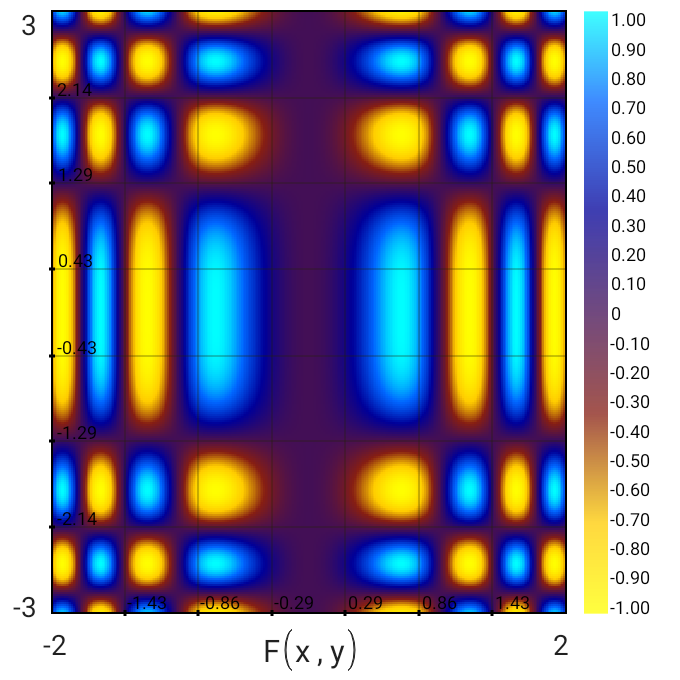
\includegraphics[resolution=320]{graphics/three_d_plot_fig2.png} \end{tabular}\end{center}

The plot boundaries, plot size and
style, labels and grid can be adjusted
by analogy with the function plot
using the plot settings dialog (see
''Function Plot'' example from the app
navigation drawer for more details).
To open this dialog, long click on the
plot area until the floating button
''Object properties'' will appear, and
than click this button.

Additionally, you can change the
number of labels along z-axis and
choose the color palette in the ''Color
Map Settings'' dialog. This dialog
appears by long click on the z-axis
bar on the right of main graph area.
\begin{center}\begin{tabular}{c}
  $R(x,y) := sin \left( 5 \cdot {x}^{2} \cdot \left( y - x \right)\right) $
\end{tabular}\end{center}
\begin{center}\begin{tabular}{c} 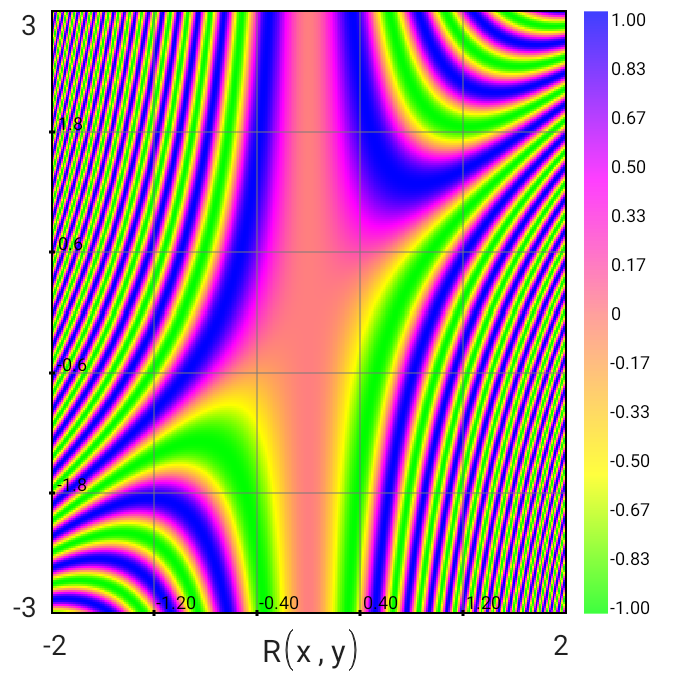
\includegraphics[resolution=320]{graphics/three_d_plot_fig3.png} \end{tabular}\end{center}

A function of two arguments can be also
plotted as a surface in 3D space. This
mode can be activated in the ''Plot
Settings'' dialog that appears if you
click floating button ''Object
properties'' after long clicking on the
plot area. Let us plot the following
function, using arrays in order to
improve calculation time:
\begin{center}\begin{tabular}{cccc}
  $N := 100$ &
  $n := \left[ 0,\, 1 \,..\, N \right]$ &
  $x1 := -15$ &
  $x2 := 15$ \cr
\end{tabular}\end{center}
\begin{center}\begin{tabular}{cccc}
  $M := 100$ &
  $m := \left[ 0,\, 1 \,..\, M \right]$ &
  $y1 := -15$ &
  $y2 := 15$ \cr
\end{tabular}\end{center}
\begin{center}\begin{tabular}{c}
  $x[n] := {\left( x1 +  \left( x2 - x1\right)  \cdot n / N \right)}^{2}$
\end{tabular}\end{center}
\begin{center}\begin{tabular}{c}
  $y[m] := {\left( y1 +  \left( y2 - y1\right)  \cdot m / M \right)}^{2}$
\end{tabular}\end{center}
\begin{center}\begin{tabular}{c}
  $r[n,m] := 0.04 \cdot x_{n}  + 0.02 \cdot y_{m} $
\end{tabular}\end{center}
\begin{center}\begin{tabular}{c}
  $t[n,m] := \left( x_{n}  + 0.05 \cdot y_{m}  \right) \cdot exp \left( 1 - r_{n,\, m} \right) $
\end{tabular}\end{center}
\begin{center}\begin{tabular}{c}
  $F[n,m] := \frac{sin \left( x_{n}  + 0.1 \cdot y_{m} \right) }{0.15 + r_{n,\, m} } + \frac{t_{n,\, m} }{10}$
\end{tabular}\end{center}
\begin{center}\begin{tabular}{c} 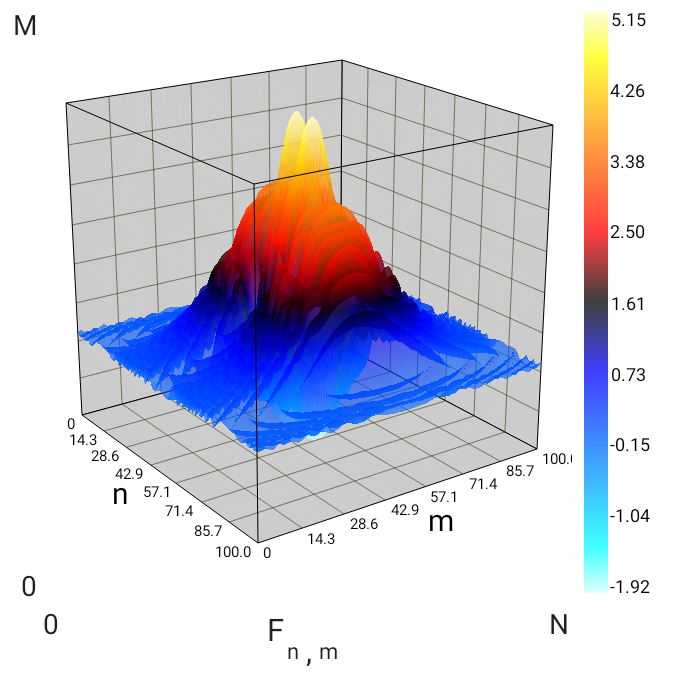
\includegraphics[resolution=320]{graphics/three_d_plot_fig4.png} \end{tabular}\end{center}

For the surface plot, there are
additional settings presented in the
''Plot Settings'' dialog. You can choose
whether the mesh lines shall be shown,
select the opacity for mesh color,
define the rotation and elevation
angles of the plot box. For example,
the previous surface plotted with
other rotation and elevation angles
looks like this: 
\begin{center}\begin{tabular}{c} 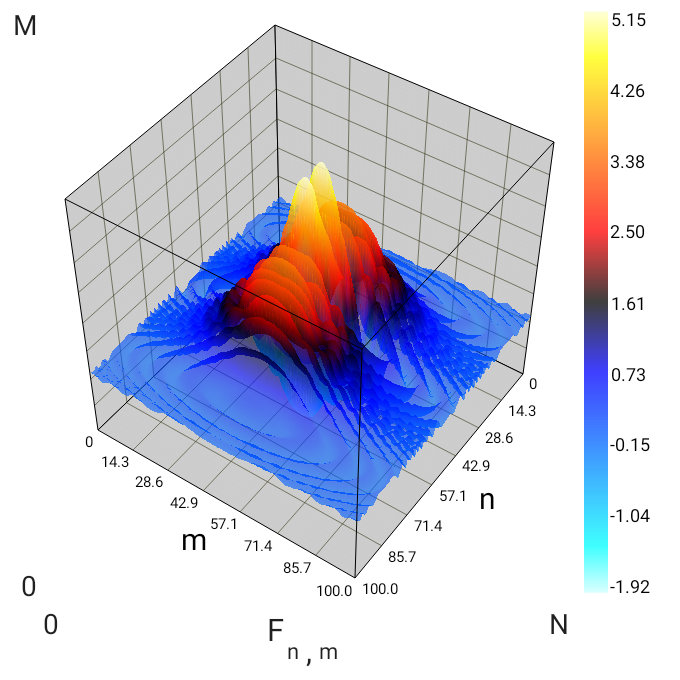
\includegraphics[resolution=320]{graphics/three_d_plot_fig5.png} \end{tabular}\end{center}

\section{Example: Series and Integrals}
% This is auto-generated file: do not edit!
% Exported from microMathematics Plus, version 2.15.4a


This example demonstrates how to
calculate series and integrals.

\subsection{Taylor series}

In mathematics, Taylor series is a
representation of a function as an
infinite sum of terms that are
calculated from the values of the
function's derivatives at a single
point.

For example, Ts(x,N) is the Taylor
expansion as a function of argument x
and the number of terms N:
\begin{center}\begin{tabular}{c}
  $Ts(x,N) := \displaystyle\sum_{n=0}^{N} \frac{{ \left( -1\right) }^{n}}{\left( 2 \cdot n \right)! } \cdot {x}^{2 \cdot n}$
\end{tabular}\end{center}

This expansion approximates the cosine
function:
\begin{center}\begin{tabular}{c}
  $s(x) := cos \left( x\right) $
\end{tabular}\end{center}

If we plot both functions together for
the same interval, they look both
equal:
\begin{center}\begin{tabular}{c}
  $x := \left[ 0,\, 0.1 \,..\, 2 \cdot {\pi} \right]$
\end{tabular}\end{center}
\begin{center}\begin{tabular}{c} 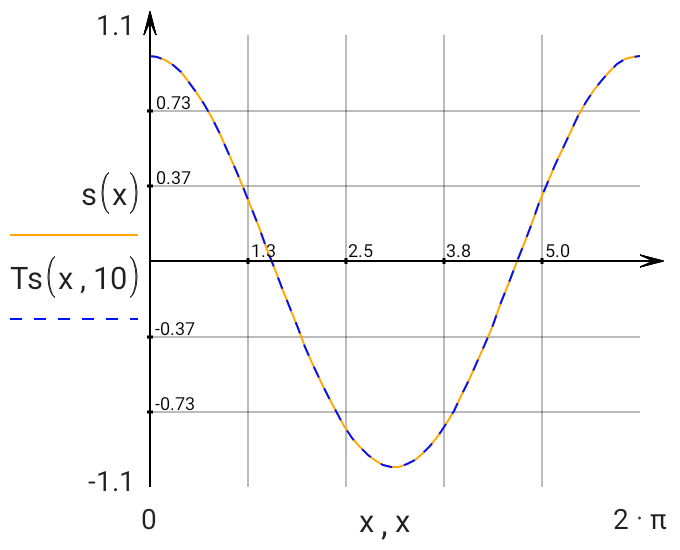
\includegraphics[resolution=320]{graphics/series_and_integrals_fig1.png} \end{tabular}\end{center}

However, there is a numerical error due
to limited number of approximation
terms N. The following function $\Delta$(x,N)
describes this error:
\begin{center}\begin{tabular}{c}
  ${\Delta}(x,N) :=  \left| s \left( x\right)  - Ts \left( x,\, N\right)  \right| $
\end{tabular}\end{center}

We can plot this function in
logarithmic coordinates and see that
the numerical error will be decreased
if we get more terms into the Taylor
summation:
\begin{center}\begin{tabular}{c}
  $E(N) := log10 \left( {\Delta} \left( {\pi},\, N\right) \right) $
\end{tabular}\end{center}
\begin{center}\begin{tabular}{c}
  $N := \left[ 3,\, 4 \,..\, 13 \right]$
\end{tabular}\end{center}
\begin{center}\begin{tabular}{c} 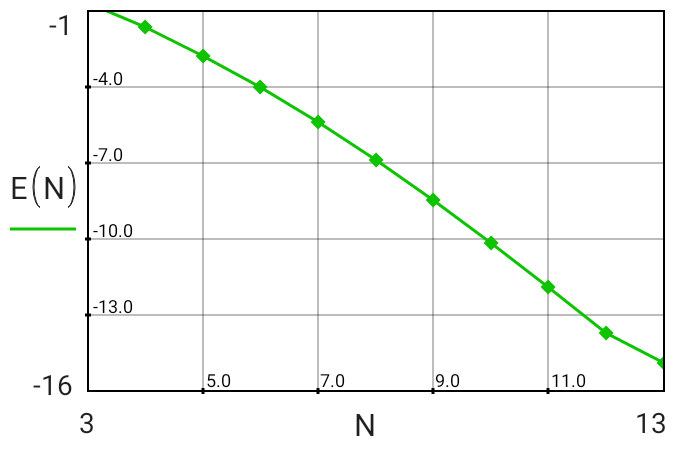
\includegraphics[resolution=320]{graphics/series_and_integrals_fig2.png} \end{tabular}\end{center}

\subsection{Binomial series}

Let us consider this power function:
\begin{center}\begin{tabular}{c}
  $f(x,{\alpha}) := {\left( 1 + x \right)}^{{\alpha}}$
\end{tabular}\end{center}

This function can be approximated using
Binomial series:
\begin{center}\begin{tabular}{c}
  $Tf(x,{\alpha},N) := \displaystyle\sum_{n=0}^{N}  \left( \displaystyle\prod_{k=1}^{n} \frac{{\alpha} - k + 1}{k}\right)  \cdot {x}^{n}$
\end{tabular}\end{center}

We can also plot both functions (the
given power function and its
approximation) together on the same
plot:
\begin{center}\begin{tabular}{c} 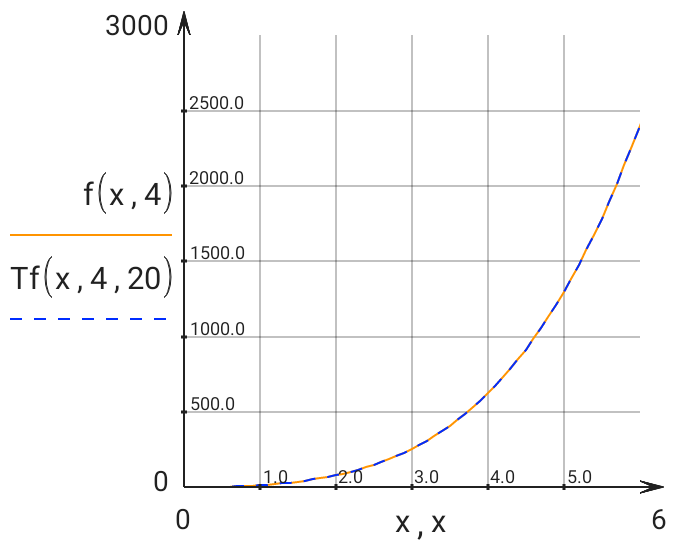
\includegraphics[resolution=320]{graphics/series_and_integrals_fig3.png} \end{tabular}\end{center}

\subsection{Integrals}

It is also possible to calculate a
definite integral numerically using
Simpson method. For example, we can
calculate the integral using ''Result
View'' element:
\begin{center}\begin{tabular}{c}
  $\displaystyle\int_{0}^{3 \cdot pi / 2}{cos \left( \frac{2 \cdot x}{9}\right) }^{-2}\, dx = 7.79423$
\end{tabular}\end{center}

The analytical solution is
\begin{center}\begin{tabular}{ccc}
  $I := \frac{9 \cdot \sqrt{3} }{2}$ &
  ,    &
  $I = 7.79423$ \cr
\end{tabular}\end{center}

Numerical error can be calculated as:
\begin{center}\begin{tabular}{c}
  $\displaystyle\int_{0}^{3 \cdot pi / 2}{cos \left( \frac{2 \cdot x}{9}\right) }^{-2}\, dx - I = 4.26681E-9$
\end{tabular}\end{center}

This error depends on the value
''Significant digits in result'' that
can be changed in the ''Document
Settings'' dialog available from the
action bar:
\begin{center}\begin{tabular}{c} 
\includegraphics[resolution=320]{graphics/series_and_integrals_fig4.png} \end{tabular}\end{center}

If this value increased, the threshold
that controls the Simpson method
precision will also be increased.

\section{About}
% This is the second part of the file about_micromath.tex
\subsection{Authors}

\begin{enumerate}
\item Mikhail Kulesh,
mikhail.kulesh@gmail.com

\item Caio Roberto Ramos da Silva
(Brazilian Portuguese translation),
caiorrs@gmail.com
\end{enumerate}

\subsection{The app icon}

The app icon is generated from the
following function defined in the
polar coordinate system:
\begin{center}\begin{tabular}{c}
  $f := \left[ 0.01,\, 0.03 \,..\, 150 \right]$
\end{tabular}\end{center}
\begin{center}\begin{tabular}{c}
  $s(f) := 4 + sin \left( 5 \cdot f\right)  + \frac{sin \left( 10 \cdot f\right) }{2} + \frac{sin \left( 60 \cdot f\right) }{6}$
\end{tabular}\end{center}
\begin{center}\begin{tabular}{c}
  $r(f) := 0.9 \cdot \left( 1 + f / 50 \right) \cdot s \left( f\right) $
\end{tabular}\end{center}
\begin{center}\begin{tabular}{c}
  $x(f) := r \left( f\right)  \cdot cos \left( f\right) $
\end{tabular}\end{center}
\begin{center}\begin{tabular}{c}
  $y(f) := r \left( f\right)  \cdot sin \left( f\right) $
\end{tabular}\end{center}
\begin{center}\begin{tabular}{c} 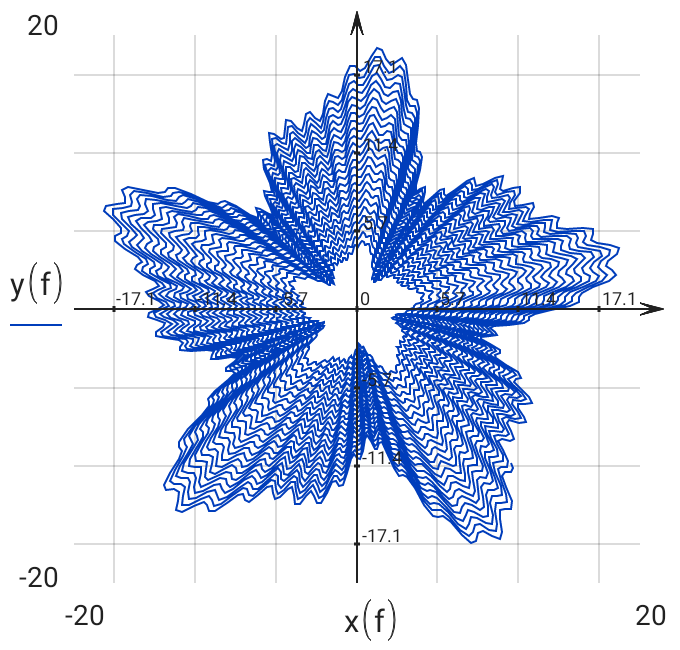
\includegraphics[resolution=320]{graphics/about_micromath_fig1.png} \end{tabular}\end{center}

2014-2017, Bremen, Germany
\end{document}